% Prepared by Calvin Kent
%
% Assignment Template v19.02
%
%%% 20xx0x/MATHxxx/Crowdmark/Ax
%
\documentclass[12pt]{article} %
\usepackage{CKpreamble}
\usepackage{CKassignment}
\usepackage{tkz-euclide}
\usepackage{physunits}
\usepackage{physics}
\usepackage{lmodern}
\usepackage{microtype}
\usepackage{tasks}
\usepackage{upgreek}
\usepackage{xcolor}
\usepackage{euscript}
\usepackage{tasks}
\usepackage{tkz-euclide}
\usepackage{upgreek}
\usepackage[misc]{ifsym}


\usepackage{pgfplots}
\usepgfplotslibrary{polar}
\usepgflibrary{shapes.geometric}
\usetikzlibrary{calc}


\usepackage{euscript}
\usepackage{microtype}
\usepackage{upgreek}
\usepackage[misc]{ifsym}

%%Title
\title{Functions Test 2 - SOLUTIONS}
\date{January 17, 2021}

%%% Maths and science packages

\usepackage{amsmath,amsthm,amssymb}
\usepackage{pgfplots}
	\usetikzlibrary{
		calc,
		patterns,
		positioning
	}
	\pgfplotsset{
		compat=1.16,
		samples=200,
		clip=false,
		my axis style/.style={
			axis x line=middle,
			axis y line=middle,
			legend pos=outer north east,
			axis line style={
				->,
			},
			legend style={
				font=\footnotesize
			},
			label style={
				font=\footnotesize
			},
			tick label style={
				font=\footnotesize
			},
			xlabel style={
				at={
					(ticklabel* cs:1)
				},
				anchor=west,
				font=\footnotesize,
			},
			ylabel style={
				at={
					(ticklabel* cs:1)
				},
				anchor=west,
				font=\footnotesize,
			},
			xlabel= $x$,
			ylabel=$\vec d (\m \tx{[East]})$
		},
	}
	\tikzset{
		>=stealth
	}

\pgfplotsset{my style/.append style={axis x line=middle, axis y line=
middle, xlabel={$t$}, ylabel={$y[\text{m}]$}, axis equal }}


%%% Tables and figures packages

\usepackage{float}
\usepackage{caption}
	\captionsetup{
		format=plain,
		labelfont=bf,
		font=small,
		justification=centering
	}
	
%%% Numbers and sets

\newcommand{\E}{\mathrm{e}}

\newcommand{\tx}[1]{\text{#1}}

\begin{document}
    \pagenumbering{arabic}
    % Start of class settings ...
    \renewcommand*{\coursecode}{MCR3U Quiz} % Quiz Title
    \renewcommand*{\assgnnumber}{1} % Quiz number
    \renewcommand*{\submdate}{November, 2021} % renew the date
    \renewcommand*{\studentfname}{\textbf{Name:}} % Student first name
    \renewcommand*{\studentlname}{} % Student last name
    %\renewcommand*{\studentnum}{SNumber} % Student number

    \renewcommand\qedsymbol{$\blacksquare$}
    \setfigpath
    % End of class settings 
    \newgeometry{left=18mm, right=18mm, top=22mm, bottom=22mm} % page is set to default values
    \fancyhfoffset[L,O]{0pt} % header orientation fixed
    % End of class settings
    %%% Note to user:
    % CTRL + F <CHANGE ME:> (without the angular brackets) in CKpreamble to specify graphics paths accordingly.
    % The command \circled[]{} accepts one optional and one mandatory argument.
    % Optional argument is for the size of the circle and mandatory argument is for its contents.
    % \circled{A} produces circled A, with size drawn for letter A. \circled[TT]{A} produces circled A with size drawn for TT.
    % https://github.com/CalvinKent/My-LaTeX
    %%%
    % Crowdmark assignment start


    %%%%%%%%%%%%%%%%%%%%%%%%%%%%%%%%%%%%%%%%%%%%%%%%%%%%%%%%%%%%%%%%%%%%%%%%%%%%%%%%%%%%%%%%%%%%%%%%%%%%%%%%
    %%%%%%%%%%%%%%%%%                  PROBLEM IDEAS                  %%%%%%%%%%%%%%%%%%%%%%%%%%%%%%%%%%%%%%
    %%%%%                   ----------------------------------------                                %%%%%%%%

    % --> Do a hard tangent line problem

	\maketitle
	\section{Preamble}
	This is a test covering what we have learnt so far in lecture. Student's \emph{\textbf{must show all work}} to receive full marks.
	\section{Allowed Aids}
	The following aids are allowed on the Test
	\begin{itemize}
    \item \textbf{Open Book Test} (Your entire binder is allowed).
	\end{itemize}
	\section{Restrictions:}
  \begin{itemize}
		\item \textbf{NO} calculator's.
  \end{itemize}
  \section{Remarks:}
  \begin{itemize}
    \item $n\cdot \textbf{S} = \underbrace{\textbf{S} + \dots + \textbf{S}}_{\text{n times}}$. \hfill $(n \in
      \mathbb N)$
    \item $\operatorname{len}(\textbf{S})$ is number of bits in the binary string $\textbf{S}$.
    \item $\operatorname{floor}(x)$ is the smallest integer less than or equal to $x$.
  \end{itemize}
	\section{Name and Date:}
	Print your name and todays date below;

  \vspace*{0.4cm}

	\begin{center}
	\noindent\begin{tabular}{ll}
		\makebox[3in]{\hrulefill} & \makebox[3in]{\hrulefill}\\
		Name & Date\\[8ex]% adds space between the two sets of signatures
	\end{tabular}
	\end{center}
	\newpage


\section*{Part A - Multiple Choice}
\begin{qstn} % qnumber, qname, qpoints
  Answer the following True/False questions,
  \begin{enumerate}
    \item Let $\operatorname{id}_\R \colon \R \to \R$ be the identity function on $\R$, then
       \[
              \operatorname{id}_\R\left(\operatorname{id}^{-1}_\R\left(\operatorname{id}_\R\left(\operatorname{id}^{-1}_\R\left(\operatorname{id}_\R\left(\operatorname{id}^{-1}_\R\left(-4
              \right) \right) \right) \right) \right) \right) = 4
      .\] 
       \textbf{\emph{Answer}}:\,\, \textbf{True} \,\,\,\,\,\, \framebox[0.5in]{\textbf{False}}\, , \,
          Note that $\operatorname{id}^{-1}_\R = \operatorname{id}_\R$.

    \item Let $f \colon \R \to \R$, $f(x) = 2(x - 1)^2$ be a function. Then $f$ is not invertible. \\
      \textbf{Hint: }Try using the Horizontal line test.\\
       \textbf{\emph{Answer}}:\,\, \framebox[0.5in]{\textbf{True}} \,\,\,\,\,\, \textbf{False}\, , \,
          Follow the hint and try using the horizontal line test to see why.

    \item Let $ \mathcal{X} = \{0.5, \pi, 3.8\} $ and $ \mathcal{Y} = \{1,4,4.8\} $ be sets, define the
            following function, 
            \begin{itemize}
              \item $\mathcal{\psi} \colon \mathcal{X} \to \mathcal{Y}$.
              \item $\mathcal{\psi}(x) = \operatorname{floor}(x) + 1$.
            \end{itemize}
            Then $\psi$ is an invertible function.\\
       \textbf{\emph{Answer}}:\,\, \textbf{True} \,\,\,\,\,\, \framebox[0.5in]{\textbf{False}}\, , \,
        Draw a mapping diagram to see why.

   \item Let $ \EuScript{S} = \{10,1100, 111000\} $ be a set of $\textit{binary strings}$ and $ Y =
     \{5,7,3\} $ be a set of natural numbers, define the following function, 
              \begin{itemize}
                \item $\Delta \colon \EuScript{S} \to Y$.
                \item $\Delta(\textbf{S}) = \operatorname{len}(\textbf{S}) + 1$.
              \end{itemize}
              Then the function,
              \begin{itemize}
                \item $\Delta^{-1} \colon Y \to \EuScript{S}$.
                \item $\Delta^{-1}(y) = \operatorname{floor}(y / 2)\cdot \textbf{1} + \operatorname{floor}(y /
                  2)\cdot \textbf{0}$,
                  \,\,\,\,(where $\textbf{1}$ and $\textbf{0}$ are $\textit{binary strings}$),
              \end{itemize}
              is the inverse function for $\Delta$.\\
       \textbf{\emph{Answer}}:\,\, \framebox[0.5in]{\textbf{True}} \,\,\,\,\,\, \textbf{False}\,
        

    \item Let $g(x) = \sqrt{x - 4} - 1$ be a function, then $g^{-1}(x) = (x-1)^2 + 4 $ is the inverse of
      $g$.\\
       \textbf{\emph{Answer}}:\,\, \textbf{True} \,\,\,\,\,\, \framebox[0.5in]{\textbf{False}}\, , \,
          $g^{-1}(x) = (x + 1)^2 + 4$

    \item Let $f(x) = x^2 $. Suppose we apply the following transformations to $f$,
      \begin{itemize}
        \item Reflection across the y-axis.
        \item Vertical compression by a factor of $3$. 
        \item Horizontal compression by a factor of $2$.
        \item Horizontal shift, left by $2$ units.
        \item Vertical shift, down by $2$ units.
      \end{itemize}
      Then the corresponding transformation equation is $h(x) = \frac{1}{3}f(-2x - 4) - 2$.\\
       \textbf{\emph{Answer}}:\,\, \framebox[0.5in]{\textbf{True}} \,\,\,\,\,\, \textbf{False}\,

    \newpage

    \item Let $f(x) = \left|x\right|$, and let $h(x) = -2f(5x - 3) + 9$ be a transformation of $f(x)$, then the
      corresponding coordinate transformation of $f$ is,
       \[
           \left( x,f(x) \right)  \longrightarrow \left( \frac{x - 3}{5}, -2f(x) + 9 \right) 
      .\] 
       \textbf{\emph{Answer}}:\,\, \textbf{True} \,\,\,\,\,\, \framebox[0.5in]{\textbf{False}}\, , \,
          The coordinate transformation is $\left( (x + 3) / 5, -2f(x) + 9 \right)$

    \item Let $\Omega \colon \mathcal{H} \to \mathcal{T}$ be a $\textit{surjective function}$, then $
      \left|\mathcal{H}\right| = \left|\mathcal{T}\right|$.\\
       \textbf{\emph{Answer}}:\,\, \textbf{True} \,\,\,\,\,\, \framebox[0.5in]{\textbf{False}}\,

    \item Let $f(x) = x^2$ , let $h(x) = -f(x)$ be a transformation of $f$, and let $r(x) = -h(-x)$ be a
      transformation of $h$, then  $r(x) = f(x)$.\\
       \textbf{\emph{Answer}}:\,\, \framebox[0.5in]{\textbf{True}} \,\,\,\,\,\, \textbf{False}\, , \, Note that
       $h(x)$ is a reflection of $f$ across the $x$-axis. $r(x)$ reflects $h$ back through the x-axis, and hence
       $f$ returns to its original position, $r(x)$ then reflects $h$ through the $x$-axis, however this has no
       effect on $x^2$ due to its symmetry.

    \item Let $f \colon \mathbb N \to \R$, $f(x) = x^2$ be a function. Then $f$ is not invertible. \\
       \textbf{\emph{Answer}}:\,\, \textbf{True} \,\,\,\,\,\, \framebox[0.5in]{\textbf{False}}\,,\, This one was
       tricky, notice that the domain is $\mathbb N$ so this function will look different from a 
       standard parabola. We'll take this up in class.



  \end{enumerate}
\end{qstn}

\newpage

\section*{Part B - Solve all problems}

\begin{qstn}
  For each of the following, you are given a function and its definition. For each question,
  \begin{enumerate}[label=(\alph*)]
    \item[(i)] Prove that the function is invertible \textbf{or} prove that the function is not invertible.
    \item[(ii)] Determine the range of the function.
  \end{enumerate}

  \begin{enumerate}[label=(\alph*)]
  \item Let $\EuScript{S} = \{1100,0011,1010\} $, $\EuScript{T} = \{0011,1010,0100,1100\}$ be sets of binary
    strings and define,
    \begin{itemize}
      \item $\lambda \colon \EuScript{S} \to \EuScript{T}$.
      \item $\lambda(\textbf{S}) = \vb s_3\vb s_4\vb s_1 \vb s_2$.
  \end{itemize}

  \begin{solution} \texttt{  }
    \begin{enumerate}[label=(\alph*)]
      \item[(i)] \texttt{  }
          \begin{center}
           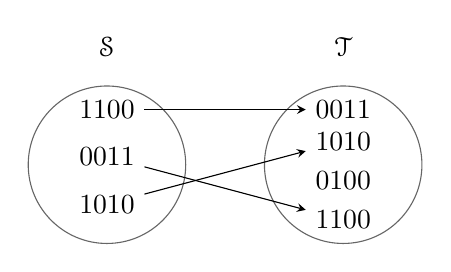
\begin{tikzpicture}
              % draw the sets
              \filldraw[fill=white!20, draw=black!60] (-1.5,0) circle (1cm);
              \filldraw[fill=white!20, draw=black!60] (1.5,0) circle (1cm);


              % the texts
              \node at (-1.5,1.5) {$\EuScript{S}$};
              \node at (1.5,1.5) {$\EuScript{T}$};

              % the points in the sets (here I just create nodes to use them later on to position
              % the circles and the arrows
              \node (x1) at (-1.5,0.7) {$1100$};
              \node (x2) at (-1.5,0.1) {$0011$};
              \node (x3) at (-1.5,-0.5) {$1010$};
              \node (y1) at (1.5,0.7) {$0011$};
              \node (y2) at (1.5,0.3) {$1010$};
              \node (y3) at (1.5,-0.2) {$0100$};
              \node (y4) at (1.5,-0.7) {$1100$};

              % draw the arrows
              \draw[->] (x1) -- (y1);
              \draw[->] (x2) -- (y4);
              \draw[->] (x3) -- (y2);

          \end{tikzpicture}
        \end{center}
        From the mapping diagram, we conclude that since $0100 \in \EuScript{T}$ is not mapped to, $\lambda$ fails
        to be surjective, since  $\lambda$ fails to be surjective, it fails to be invertible.

      \item[(ii)] Based on the outputs given in the mapping diagram, we conclude that the range of the function is,
        \[
            \mathcal{R}_\lambda = \{0011,1010,1100\} 
        .\] 
    \end{enumerate}
  \end{solution}





  \item Let $\mathcal{N} = \{2.7,0.2,1.3,2.4\} $, $\mathcal{M} = \{0,2,4\}$ be sets and define,
    \begin{itemize}
      \item $\omega \colon \mathcal{N} \to \mathcal{M}$.
      \item $\omega(n) = 2\cdot \operatorname{floor}(n)$.
    \end{itemize}

  \begin{solution} \texttt{  }
    \begin{enumerate}[label=(\alph*)]
      \item[(i)] \texttt{  }
          \begin{center}
           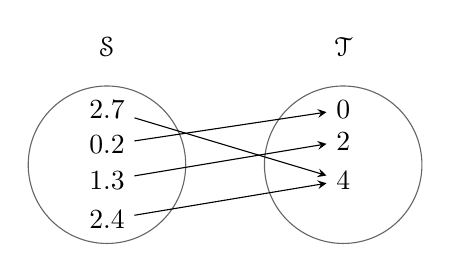
\begin{tikzpicture}
              % draw the sets
              \filldraw[fill=white!20, draw=black!60] (-1.5,0) circle (1cm);
              \filldraw[fill=white!20, draw=black!60] (1.5,0) circle (1cm);


              % the texts
              \node at (-1.5,1.5) {$\EuScript{S}$};
              \node at (1.5,1.5) {$\EuScript{T}$};

              % the points in the sets (here I just create nodes to use them later on to position
              % the circles and the arrows
              \node (x1) at (-1.5,0.7) {$2.7$};
              \node (x2) at (-1.5,0.25) {$0.2$};
              \node (x3) at (-1.5,-0.2) {$1.3$};
              \node (x4) at (-1.5,-0.7) {$2.4$};
              \node (y1) at (1.5,0.7) {$0$};
              \node (y2) at (1.5,0.3) {$2$};
              \node (y3) at (1.5,-0.2) {$4$};

              % draw the arrows
              \draw[->] (x1) -- (y3);
              \draw[->] (x2) -- (y1);
              \draw[->] (x3) -- (y2);
              \draw[->] (x4) -- (y3);

          \end{tikzpicture}
        \end{center}
        From the mapping diagram, we conclude that since $\omega(2.7) = \omega(2.4) = 4$, $\omega$ fails
        to be injective, since  $\omega$ fails to be injective, it fails to be invertible.

      \item[(ii)] Based on the outputs given in the mapping diagram, we conclude that the range of the function is,
        \[
            \mathcal{R}_\omega = \{0,2,4\} 
        .\] 
    \end{enumerate}
  \end{solution}
  \end{enumerate}

\end{qstn}

\newpage

\begin{qstn}
  Let $\beta \colon V \to W$ be an invertible function. Suppose that the formula for the invertible function is,
  \[
      \beta^{-1}(w) = 2w - 4
  .\] 
  \begin{enumerate}[label=(\alph*)]
    \item Given the co-domain $W = \{-2,-4,0,2\} $ of $\beta$, recover the domain $V$.
      \begin{solution}
        Since $\beta$ is invertible, each element in the domain $V$ corresponds to a unique element in the
        co-domain $W$, the inverse function  $\beta^{-1}$ allows us to remap each element in $W$ to its unique
        corresponding element in the domain $V$. Hence, it suffices to determine the output of $\beta^{-1}(w)$ for
        each $w \in W$. \textbf{(Ask me in class if you are still confused)}

        \begin{center}
          \begin{tabular}{c|c}
          \text{$W$} & \text{$\beta^{-1}(w)$}\\\hline 
            $-2$ & $\beta^{-1}(-2) =  2(-2) - 4 = -8$\\
            $-4$ & $\beta^{-1}(-4) =  2(-4) - 4 = -12$\\
            $0$ & $\beta^{-1}(0) =  2(0) - 4 = -4$\\
            $2$ & $\beta^{-1}(2) =  2(2) - 4 = 0$
          \end{tabular}
         \end{center}
         And hence $V = \{-12,-8,-4,0\} $.
      \end{solution}


  \item Determine the formula for $\beta(v)$.\\
    \textbf{Hint: }Use the same algorithm for determining the inverse.
    \begin{solution}
      Proceeding with the inverse algorithm,
      \begin{align*}
        \beta^{-1}(w) &= 2w - 4\\
              y &= 2w - 4\\
              y + 4 &= 2w\\
              w &= \frac{1}{2}(w + 4)\\
              \beta(v) &= \frac{1}{2}(v + 4)
      .\end{align*}
    \end{solution}


  \item Confirm that your formula for $\beta(v)$ is correct by checking that each element in $V$ correctly maps back to the corresponding
        elements in $W$.
        \begin{solution}
          To do so we proceed with a table of outputs,
            \begin{center}
              \begin{tabular}{c|c}
              \text{$V$} & \text{$\beta(v)$}\\\hline 
                $-12$ & $\beta(-12) =  (-12 + 4) / 2 = -4$\\
                $-8$ & $\beta(-8) =  (-8 + 4) / 2 = -2$\\
                $-4$ & $\beta(-4) =  (-4 + 4) / 2 = 0$\\
                $0$ & $\beta(0) =  (0 + 4) / 2 = 2$
              \end{tabular}
             \end{center}
            By the table of outputs, we conclude that each element in $V$ maps to the correct corresponding 
            element in $W$. And hence we have certificate of correctness for our formula for $\beta$.

        \end{solution}

  \end{enumerate}
\end{qstn}

\newpage

\begin{qstn}
Let $ X = \{-3,0,-5\} $ and $ Y = \{5,3,0\} $ be sets, define the following function, 
\begin{itemize}
    \item $\Phi \colon X \to Y$.
    \item $\Phi(x) = \left|x\right|$.
\end{itemize}

Prove that the function,
\begin{itemize}
    \item $\Phi^{-1} \colon Y \to X$.
    \item $\Phi^{-1}(y) = -\operatorname{id}_Y(y)$.
\end{itemize}
is the inverse function for $\Phi$.

\begin{solution}
  We confirm that both conditions of Definition 4.1 hold with mapping tables,
  \begin{center}
    \begin{tabular}{c|c}
  \text{$X$} & \text{$\Phi^{-1}\left( \Phi(x) \right) $}\\\hline 
        $-3$ & $\Phi^{-1}\left( \Phi(-3) \right) =  \Phi^{-1}\left( 3 \right) = -\operatorname{id}_Y(3) = -3$\\
        $0$ & $\Phi^{-1}\left( \Phi(0) \right) =  \Phi^{-1}\left( 0 \right) = -\operatorname{id}_Y(0) = 0$\\
        $-5$ & $\Phi^{-1}\left( \Phi(-5) \right) =  \Phi^{-1}\left( 5 \right) = -\operatorname{id}_Y(5) = -5$
 	\end{tabular}

    \begin{tabular}{c|c}
  \text{$Y$} & \text{$\Phi\left( \Phi^{-1}(y) \right) $}\\\hline 
        $5$ & $\Phi\left( \Phi^{-1}(5) \right) =  \Phi\left( -5 \right) = \left|-5\right|  = 5$\\
        $3$ & $\Phi\left( \Phi^{-1}(3) \right) =  \Phi\left( -3 \right) = \left|-3\right|  = 3$\\
        $0$ & $\Phi\left( \Phi^{-1}(0) \right) =  \Phi\left( 0 \right) = \left|0\right|  = 0$
 	\end{tabular}
\end{center}
By our results from the mapping tables, we conclude that $\Phi^{-1}(y) = -\operatorname{id}_Y$ is indeed the inverse function
for $\Phi$.
\end{solution}


\end{qstn}

  
\newpage


\begin{qstn}
  Determine the inverse function for the following functions,
  \begin{enumerate}[label=(\alph*)]
    \item $f(x) = 4x + 8$.
      \begin{solution}
        Proceeding with the inverse algorithm,
        \begin{align*}
              f(x) &= 4x + 8\\
              y &= 4x + 8\\
              y - 8 &= 4x\\
              x &= \frac{1}{4}(y - 8)\\
              f^{-1}(x) &= \frac{1}{4}(x - 8)
        .\end{align*}
      \end{solution}

      \vspace*{2cm}

    \item $H(x) = \sqrt{x - 16} + 2$.
      \begin{solution}
        Proceeding with the inverse algorithm,
        \begin{align*}
          H(x) &= \sqrt{x - 16} + 2\\
          y &= \sqrt{x - 16}  + 2\\
          y - 2 &= \sqrt{x - 16} \\
          (y - 2)^2 &= x - 16\\
          x &= (y - 2)^2 + 16\\
          f^{-1}(x) &= (x - 2)^2 + 16
        .\end{align*}
      \end{solution}
  \end{enumerate}
\end{qstn}

\newpage

\begin{qstn}
Suppose that I throw a ball from ground level and my sister simultaneously throws a rock. She manages to hit the
ball at exactly $t=  3$ seconds.
      \begin{center}
      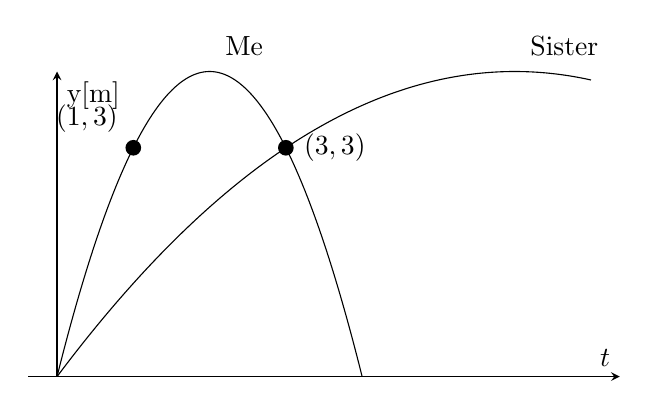
\begin{tikzpicture}
        \begin{axis}[
          my style,
          ytick=\empty,
          xtick=\empty,
          xticklabels=\empty,
          width=0.75\textwidth,
          height=0.45\textwidth,
          yticklabels=\empty,
          ylabel={y[m]}]

          \addplot[domain=0:4]{-(x -  2)^2 + 4};
          \addplot[domain=0:7]{-(0.3333333*x -  2)^2 + 4};

          \node[label={45:{\textcolor{black}{Me}}},circle,inner sep=2pt] at (axis cs:2,4) {};
          \node[label={45:{\textcolor{black}{Sister}}},circle,inner sep=2pt] at (axis cs:6,4) {};
          \node[label={0:{\textcolor{black}{$(3,3)$}}},circle,fill,inner sep=2pt] at (axis cs:3,3) {};

          \node[label={135:{\textcolor{black}{$(1,3)$}}},circle,fill,inner sep=2pt] at (axis cs:1,3) {};

        \end{axis}
      \end{tikzpicture}
      \end{center}
\end{qstn}
Let $M(x)$ denote my graph and $S(x)$ denote the graph of my sister. We can represent the graph of my sister as
a horizontal scaling of my graph, 
\begin{align*}
  S(x) = M(B\cdot x) \tag{$B \in \R, B \neq 1$}
\end{align*}
 Using the data given in the plot, determine the correct value for $B$.
 \begin{solution}[\textbf{1}]
   Since my sister hits the ball at exactly $t = 3$ seconds, it follows that $S(3) = 3$. Since $M(1) = 3$, we can
   horizontally stretch my graph $M(x)$ by a factor  $3$ to obtain,
   \[
      S(3) = M\left( \frac{1}{3}\cdot 3 \right) = M(1) = 3
   .\] And hence,
   \[
        B = \frac{1}{3}
   .\] 
 \end{solution}

 \begin{solution}[\textbf{2}]
   Another solution is to think about how to transform,
   \[
      (1,3) \longrightarrow (3,3)
   .\] After which you could conclude that a horizontal stretch by a factor of $3$ should do the job,
   \[
      (1,3) \longrightarrow \left(\frac{1}{1 / 3}, 3 \right) = (3,3) 
   .\] 
 \end{solution}




\newpage

\begin{qstn}
  Let $f(x) = \left|x\right|$, and let $R(x) = -\frac{1}{2}f(2x + 4) + 1$ be a transformation of $f$. 
  \begin{enumerate}[label=(\alph*)]
    \item Describe the transformation.
      \begin{solution}
        Let $A = -1 / 2, B = 2, H = 4, K = 1$.We first we factor $R(x)$ to obtain,
        \[
            R(x) = -\frac{1}{2}f(2x + 4) + 1 = -\frac{1}{2}f(2(x + 2)) + 1
        .\] 
        From which we can describe the transformations,
        \begin{itemize}
          \item Since $A < 0$, $f$ is reflected across the x-axis.
          \item $f$ is horizontally shifted left by $2$ units.
          \item $f$ is vertically shifted up by $1$ unit.
          \item Since $\left|A\right| = \frac{1}{2}$ and $0 < \frac{1}{2} < 1$ we conclude that $f$ has been
            vertically compressed by a factor of $2$.
          \item  Since $ \left|B\right| = 2$ and $2 > 1$ we conclude that $f$ has been horizontally compressed by a
            factor  of $2$.
        \end{itemize}
      \end{solution}

    \item Determine the expression for the coordinate transformation,
      \[
          \left( \frac{x- H}{B}, Af(x) + K \right) =
          \left( \frac{x - 4}{2}, -\frac{1}{2}f(x) + 1\right) 
      \] 
      \vspace*{1cm}

    \item Complete the following coordinate table to determine the corresponding transformed coordinates.
        \begin{center}
          \begin{tabular}{c|c}
        \text{$\left( x,f(x) \right) $} & \text{$ \left( (x - 4) / 2, -\frac{1}{2}f(x) + 1\right) $}\\\hline 
              \\
              $(0,0)$ & $(-2,1)$\\
              \\
              \\
              $(-6,6)$ & $(-5,-2)$\\
              \\
              \\
              $(6,6)$ & $(1,-2)$\\
              \\
              \\
              $(-4,4)$ & $(-4,-1)$\\
              \\
              \\
              $(4,4)$ & $(0,-1)$\\
              \\
              \\
        \end{tabular}

        \end{center}

  \newpage

   \item Using your results from the coordinate table, sketch the transformation $R(x)$. Be sure to
     \textbf{label} the transformed coordinates as well as the function.

    \begin{center}
        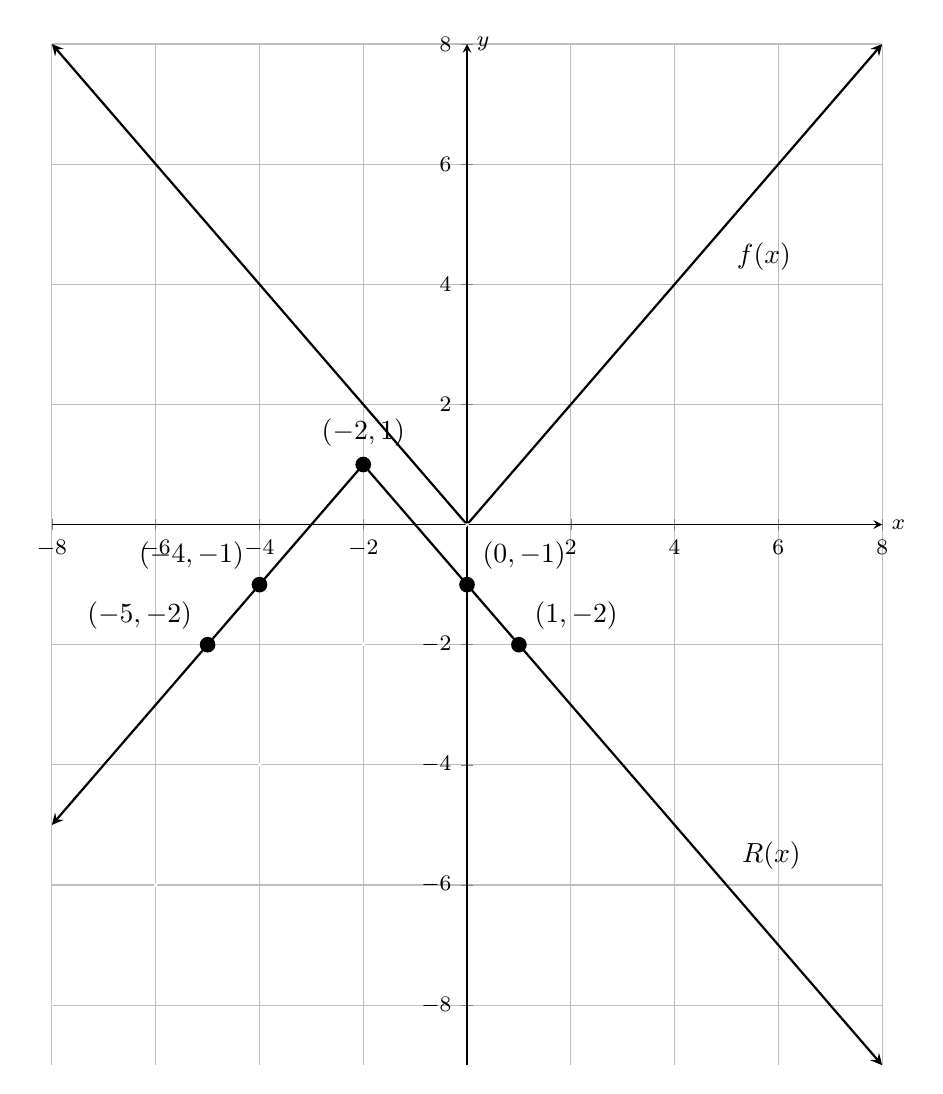
\begin{tikzpicture}
        \begin{axis}[
            my axis style,
            width=1\textwidth,
            height=1.2\textwidth,
            ylabel=$y$,
            grid
        ]
        
        \addplot[
            domain=-8:8,
            thick,
            white,
            -
        ]
        {x};
 
        \addplot[
            domain=-8:8,
            thick,
            black,
            <->
        ]
        {abs(x)};

        \addplot[
            domain=-8:8,
            thick,
            black,
            <->
        ]
        {-0.5*abs(2*x + 4) + 1};

        \fill[
            black
        ];

        \node[label={275:{\textcolor{black}{$f(x)$}}},circle,inner sep=2pt] at (axis cs:5,5) {};
        \node[label={45:{\textcolor{black}{$R(x)$}}},circle,inner sep=2pt] at (axis cs:5,-6) {};

        \node[label={90:{\textcolor{black}{$(-2,1)$}}},circle,fill,inner sep=2pt] at (axis cs:-2,1) {};
        \node[label={135:{\textcolor{black}{$(-5,-2)$}}},circle,fill,inner sep=2pt] at (axis cs:-5,-2) {};
        \node[label={135:{\textcolor{black}{$(-4,-1)$}}},circle,fill,inner sep=2pt] at (axis cs:-4,-1) {};
        \node[label={45:{\textcolor{black}{$(0,-1)$}}},circle,fill,inner sep=2pt] at (axis cs:0,-1) {};
        \node[label={45:{\textcolor{black}{$(1,-2)$}}},circle,fill,inner sep=2pt] at (axis cs:1,-2) {};

        \end{axis}
        \end{tikzpicture}
    \end{center}
  \end{enumerate}
\end{qstn}

\newpage


\section*{Part C - Solve exactly one of the three problems.} 

\begin{qstn}
  Let $A = \{a,b,c\}$, $B = \{x,y,z\}$ be sets. Let $\mathcal{L}$ be the set of all functions from $A \to B$. Let
  $\mathcal{M} = \{f \in \mathcal{L} \mid f \text{ is invertible}\} $. Determine $\left|\mathcal{M}\right|$ and
  justify that your answer is correct.\\
  \textbf{Note: }Try counting all possible mapping diagrams between $A$ and $B$. Two invertible functions are the same if their mapping diagrams are equivalent.
\end{qstn}
\begin{solution}[\textbf{1}]
  Each function $f \in \mathcal{M}$ is an invertible function between $A$ and $B$ with a unique mapping diagram
  where each element in $A$ is mapped to a unique element in $B$. Hence we can count all possible ways to
  construct such a mapping diagram. For $a \in A$, we can map it to either $x,y,z$, this gives us  $3$ choices.
  For each of those choices, we can map $b \in A$ to either of the $2$ remaining choices. And lastly, for $c \in
  A$, we can map it to the remaining single choice. This gives us a total of $6$ choices, and hence $
  \left|\mathcal{M}\right| = 6$.
\end{solution}

\begin{solution}[\textbf{2}]
  Another approach to count all possible invertible mapping diagrams between $A$ and $B$ is to draw all of them.
\end{solution}

\begin{qstn}
  Let $A,B$ be sets, and let  $F \colon A \to B$ be a function between the sets. We define the \textbf{nullset} of
  $F$ to be,
  \[
        \text{Null}(F) = \{a \in A \mid F(a) = 0\} 
  .\] 
  Let $G \colon \R \to \R$, $G(x) = 2x - 4$,
   \begin{enumerate}[label=(\alph*)]
     \item Determine $\text{Null}(G)$.
     \item What do you think $\text{Null}(G^{-1})$ contains and why?
     \item Determine $\text{Null}(G^{-1})$.
  \end{enumerate}
  \begin{solution}\texttt{   }
    \begin{enumerate}[label=(\alph*)]
      \item Note that,
        \begin{align*}
          \text{Null}(G) &= \{x \in \R \mid G(x) = 0\}\\
                         &= \{x \in \R \mid 2x - 4 = 0\} 
        .\end{align*}
        At this point we conclude that $\text{Null}(G)$ contains the solution to the equation $2x - 4 = 0$.
        If we solve the equation by isolating for $x$, we get that $x = 2$. Hence,
        \[
           \text{Null}(G) = \{2\}  
        .\] 
      \item $\text{Null}(G^{-1})$ contains the y-intercept of $G$. This is because $G(0) = 4$ is the y-intercept of
        $G$, therefore the inverse function $G^{-1}$ will map $4$ back to $0$. Hence, $G^{-1}(4) = 0$. Because $G$ 
        is invertible, $G^{-1}$ can at most map a single element back to $0$, or else it would fail to be
        injective. Hence $G^{-1}$ contains only the y-intercept of $G$.

      \item From our previous argument, we conclude that,
        \[
              \text{Null}(G^{-1}) = \{4\} 
        .\] 
    \end{enumerate}
  \end{solution}
  
\end{qstn}

\newpage

\begin{qstn}
  Consider the following grid below,
  \begin{center}
    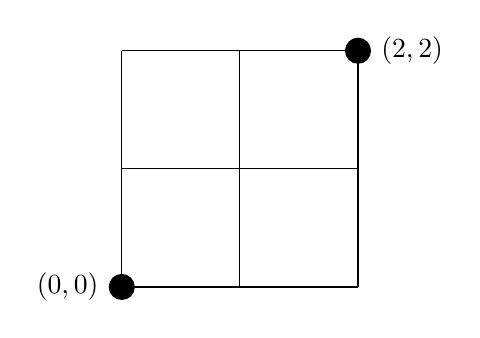
\begin{tikzpicture}
    \draw[step=1.5cm,color=black] (0,0) grid (3,3);

        \node[label={0:{\textcolor{black}{$(2,2)$}}},circle,fill] at (3,3) {};
        \node[label={180:{\textcolor{black}{$(0,0)$}}},circle,fill] at (0,0) {};

    \end{tikzpicture}
  \end{center}

  Let \texttt{R} denote a rightward move and \texttt{U} denote an upward move. We define a path from $(0,0)$ to  $(2,2)$ to be a 
  sequence of rightward and upward moves. For example \texttt{RRUU} is a path from $(0,0)$ to  $(2,2)$, and so is
  \texttt{UURR}.

  \begin{enumerate}[label=(\alph*)]
    \item Determine all paths from $(0,0)$ to  $(2,2)$. Collect all of these paths into the set $\EuScript{P}$.\\
      \textbf{Hint:} $\left|\EuScript{P}\right| = 6$.
    \item Let $Z = \left\{ \{1,2\}, \{1,3\}, \{1,4\}, \{2,3\}, \{2,4\} , \{3,4\}\right\} $.
      \begin{enumerate}[label=(\alph*)]
        \item [(i)]Describe a function $\Psi \colon \EuScript{P} \to Z$ that assigns a 
          relationship between the two sets.\\
          \textbf{Note:} The function description can be in words.
        \item [(ii)] Draw a mapping diagram for $\Psi$ based on your description of the function.\\
          \textbf{Hint:} In my description : $\Psi(\texttt{UURR}) = \{3,4\}, \Psi(\texttt{RUUR}) = \{1,4\} $
          (Yours could be different)\\

      \end{enumerate}
  \item Describe the inverse function $\Psi^{-1} \colon Z \to \EuScript{P}$.\\

  \end{enumerate}

  
\end{qstn}

\begin{solution} \texttt{  }
  \begin{enumerate}[label=(\alph*)]
    \item After counting all the paths, you should obtain,
      \[
          \mathcal{P} = \{\texttt{RURU}, \texttt{RRUU}, \texttt{RUUR}, \texttt{URRU}, \texttt{URUR}, \texttt{UURR}\} 
      .\] 
    \item 
      \begin{enumerate}[label=(\alph*)]
        \item[(i)] The function can be described as follows, for every path  $p \in \mathcal{P}$, $\Psi(p)$ assigns
          to the path $p$ the set in $Z$ which contains the integers which correspond to the positions of the
          character \texttt{R} in the path $p$. So for example, $\Psi(\texttt{URRU}) = \{2,3\} $ .
        \item[(ii)] By our description of $\Psi$ from (i), we can deduce the mapping diagram,

          \begin{center}
           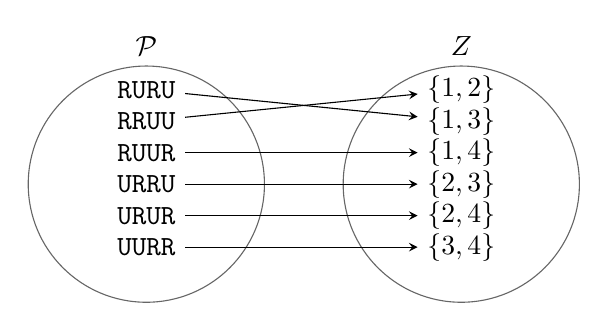
\begin{tikzpicture}
              % draw the sets
              \filldraw[fill=white!20, draw=black!60] (-2,0) circle (1.5cm);
              \filldraw[fill=white!20, draw=black!60] (2,0) circle (1.5cm);


              % the texts
              \node at (-2,1.75) {$\mathcal{P}$};
              \node at (2,1.75) {$Z$};

              % the points in the sets (here I just create nodes to use them later on to position
              % the circles and the arrows
              \node (x1) at (-2,1.2) {\texttt{RURU}};
              \node (x2) at (-2,0.8) {\texttt{RRUU}};
              \node (x3) at (-2,0.4) {\texttt{RUUR}};
              \node (x4) at (-2,0) {\texttt{URRU}};
              \node (x5) at (-2,-0.4) {\texttt{URUR}};
              \node (x6) at (-2,-0.8) {\texttt{UURR}};
              \node (y1) at (2,1.2) {$\{1,2\}$};
              \node (y2) at (2,0.8) {$\{1,3\}$};
              \node (y3) at (2,0.4) {$\{1,4\}$};
              \node (y4) at (2,0) {$\{2,3\}$};
              \node (y5) at (2,-0.4) {$\{2,4\}$};
              \node (y6) at (2,-0.8) {$\{3,4\}$};

              % draw the arrows
              \draw[->] (x1) -- (y2);
              \draw[->] (x2) -- (y1);
              \draw[->] (x3) -- (y3);
              \draw[->] (x4) -- (y4);
              \draw[->] (x5) -- (y5);
              \draw[->] (x6) -- (y6);

          \end{tikzpicture}
        \end{center}

      \end{enumerate}
    \item The inverse function can be described as follows, for every set  $S \in Z$, $\Psi^{-1}(S)$ assigns
          to the set $S$ the path in $\mathcal{P}$ which contains the character \texttt{R} at the positions
          indicated by the integers in the set $S$. So for example, $\Psi^{-1}(\{2,4\} ) = \texttt{URUR}$.
  \end{enumerate}
\end{solution}


\end{document}































